\section{Evaluation}

A large challenge in creating quality measures is the
problem of evaluating the performance of the measure.
``Quality'' is an imprecise notion by itself, because it
necessarily must be evaluated with respect to some attribute.
For example, within the Wikipedia we might evaluate the quality
of a contribution along any of these dimensions:
\begin{itemize}
\item grammar
\item diction
\item neutral point of view
\item factual correctness
\end{itemize}
Our text and edit longevity measures try to go one step
further into the fuzzy world of human evaluations by using
later edits as a basis for inferring sentiment about earlier edits.
Is this a valid inference to make?
How can such a question be answered?

The surest way to measure sentiment would be to interview
users as they are making edits to the Wikipedia and documenting
their thought processes as they read an article and make the
decision to edit an article --- but this would require an enormous
effort to collect enough data for performance evaluation.
We propose that we can grossly measure the sentiment of the
community by recognizing that there is a generally agreed upon
standard of articles being of ``encyclopedic quality''
which allows people to recognize vandalism when they see it.
Accepting that premise allows us to use the PAN-WVC-10
corpus~\cite{Potthast2010a} as a manually annotated data set for
such an evaluation.

The PAN-WVC-10 corpus was used to compare the performance of
solutions for the 1st International Competition on Wikipedia
Vandalism Detection~\cite{Potthast2010b}.
We use it in a similar way here, but with an important distinction:
we use information ``from the future'' to calculate our
quality values for the annotated revisions.
Standard vandalism detection tools make their determination
immediately as the edit is made, so that any vandalism can be
quickly repaired by others.
The necessity for a quick classification precludes waiting
for future edits or rating to corroborate the edit being judged;
we term this variation of the problem \textit{immediate vandalism detection}.
By definition, our two longevity metrics use later edits to
measure the quality of the revision being judged; we call
this the \textit{historical vandalism detection} problem.
Historical vandalism detection has applications such as selecting
high quality revisions for DVD compilations or for presentation
to school children.

The PAN-WVC-10 corpus contains 32,439 edits, where each revision was
manually reviewed by at least three annotators to assign a label
of either ``regular'' or ``vandalism.''
We used the dump of the English Wikipedia from January 30, 2010
to extract the text of each annotated revision, along with the revision
before and the ten filtered revisions following so that we could compute
our text longevity and edit longevity measures for each annotated edit.
Out of the total 32,439 revisions, we were able to compute
edit longevity scores for 27,730 revisions, and text longevity
scores for 28,453 revisions.

We used the straight-forward transformation to convert
each quality score from its normal range into the range
$[0,1]$, to be interpreted as a probability that the named
revision was the result of vandalism.
As in the PAN 2010 competition~\cite{Potthast2010b}, we use the
\texttt{perf}\footnote{\url{http://kodiak.cs.cornell.edu/kddcup/software.html}}
package to evaluate the performance of our quality measures
by computing the area under the receiver operating characteristic
curve \footnote{\url{http://en.wikipedia.org/wiki/Receiver_operating_characteristic}},
and also the mean precision value.

\subsection{Difference Algorithms}

Each formula for edit distance we have defined so far is calculated
from the operations within the edit script describing the transformation
from the source revision to the target revision.
This edit script is highly dependent on the algorithm used to
compute the difference between the revisions.
To provide a more complete picture of how the choice of difference
algorithm affects the performance of the quality measures,
we present an evaluation of two different algorithms:
\textit{greedy} and \textit{live}.
The \textit{greedy} difference algorithm is our original greedy
algorithm described in Section~\ref{sec:diff-greedy}, including
the optimizations.
The \textit{live} difference algorithm is an updated version of
our greedy algorithm that is used in the live WikiTrust system today,
with the code implementing it being available from
Github.\footnote{\url{http://www.github.com/collaborativetrust/WikiTrust}}

\subsection{Match Quality Formulas}

\mynote{Insert list here.}

\subsection{Edit Distance Formulas}

\mynote{Insert list here.}

\subsection{Results}

A complication in our evaluation is our restricted setting of
\textit{filtered} revisions, where sequential revisions by the
same author are filtered out to leave only the last revision
in the sequence.
This would limit us in evaluating the performance of our
quality measures, so we modified the system in the following way:
we do not filter revisions annotated in the PAN-WVC-10 corpus,
or the immediately preceding revision (even when they have the
same author), but we do filter revisions \textit{after} the annotated
revision in the usual way.
Even with this loosening of the revision filtering, several
revisions are still not evaluated for quality; the two
primary reasons for no evaluation are a lack of subsequent
edits to base the evaluation on, or the revision was not
substantially different from the previous revision
(that is, $\dist{}{k-1,k} = 0$, which can happen when only
whitespace changes).

\subsubsection{Edit Longevity}

Edit longevity performs quite well, at over 91\% ROC-AUC;
very close to the performance of the winning solution from
the Wikipedia Vandalism Detection competition~\cite{Potthast2010b}.
The PR-AUC is more middling, near fourth place in the competition.

This result is very encouraging, because it means that can
estimate the quality of revisions in a relatively simple way.
Knowing the quality of edits, we can build up a reputation
system for authors based on the quality of their work.


\begin{table}[tbph]
\begin{center}
\begin{tabular}{|c|c|c||c|c|c|}
\hline
Diff & Match Quality & Edit Distance & Num Revs & ROC AUC & Mean Prec \\
\hline
\hline
greedy & initial &initial distance & xx & xx & xx \\
greedy & initial &updated distance & xx & xx & xx \\
live & initial &I+D-$\frac{1}{2}$ & 27,635 & 91.758\% & 44.052\% \\
live & initial &replacements & 27,730 & 91.761\% & 46.539\% \\
\hline
\end{tabular}
\end{center}
\caption{Comparison of the performance of edit longevity
  using three different definitions of edit distance.
  The edit quality computed was used as a predictor for the probability
  that annotated revisions from the PAN-WVC-10 corpus were vandalism.
  Each measure is evaluated by computing the area under the
  receiver operating characteristic (ROC) curve.
} 
\end{table}


\subsubsection{Text Longevity}

The number of revisions is good: 28,453 / 32,439.
Text longevity is not calculated when there are no
judging editors after the revision we are computing
the text longevity for.
This argues that 28,453 is an upper bound for the number
of revisions that we are able to calculate \textit{any}
quality measure for.

The ROC-AUC of 85.9\% seems good, but ranks in seventh place
in the PAN-2010 competition.
But this is quite bad, because we're doing \textit{historical
vandalism detection}, where we use data from the future to
inform our evaluation of the revision.

The most interesting result in this table of results
is the fact that the match quality function made
nearly no difference in the predictive ability of
text longevity.

\mynote{Try mq just using length.}

\begin{table}[tbph]
\begin{center}
\begin{tabular}{|c|c||c|c|c|}
\hline
Diff & Match Quality & Num. Revisions & ROC AUC & Mean Precision \\
\hline
\hline
greedy & initial & xx & xx & xx \\
live & initial & 28,453 & 85.949\% & 29.235\% \\
\hline
\end{tabular}
\end{center}
\caption{Comparison of the performance of text longevity.
} 
\end{table}

Why does text longevity not do so well as edit longevity?
As part of our investigation, we started looking at specific
instances of text longevity values.
In Figures~\ref{fig:ts-GeorgeWBush} and~\ref{fig:ts-SantaCruzBeachBoardwalk},
we see the text survival for two different contributions;
both do seem to have the general ``exponential'' shape
that we previously described.
Also computed in each figure is the text longevity measure based on
the 20~revisions shown in each graph, but notice that the text
longevity computed for
Figure~\ref{fig:ts-GeorgeWBush} doesn't exhibit curve we expect.

\begin{figure}[tbph]
\centering
\framebox{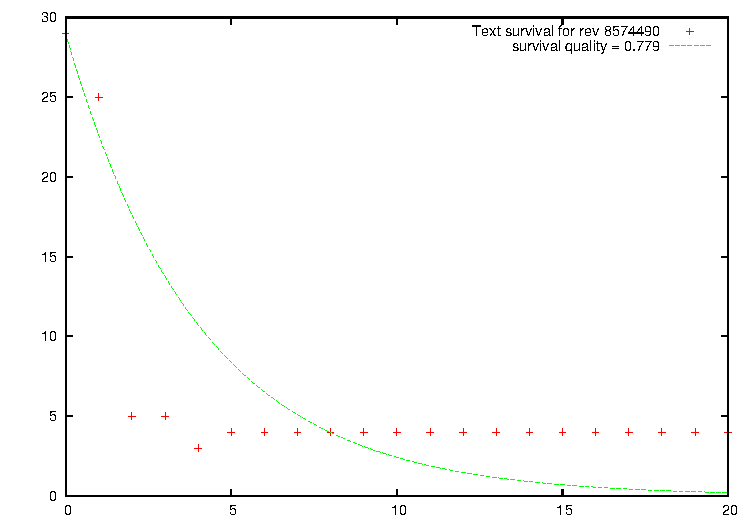
\includegraphics[width=0.8\textwidth]{part-F70-editquality/graph-TS-GeorgeWBush-8574490}}
\caption{The text survival graph for the text contributed early
        in the history of article \textit{George W.~Bush}.
	The graph also shows the text survival quality
	computed based on 20~revisions.
	}
\label{fig:ts-GeorgeWBush}
\end{figure}

\begin{figure}[tbph]
\centering
\framebox{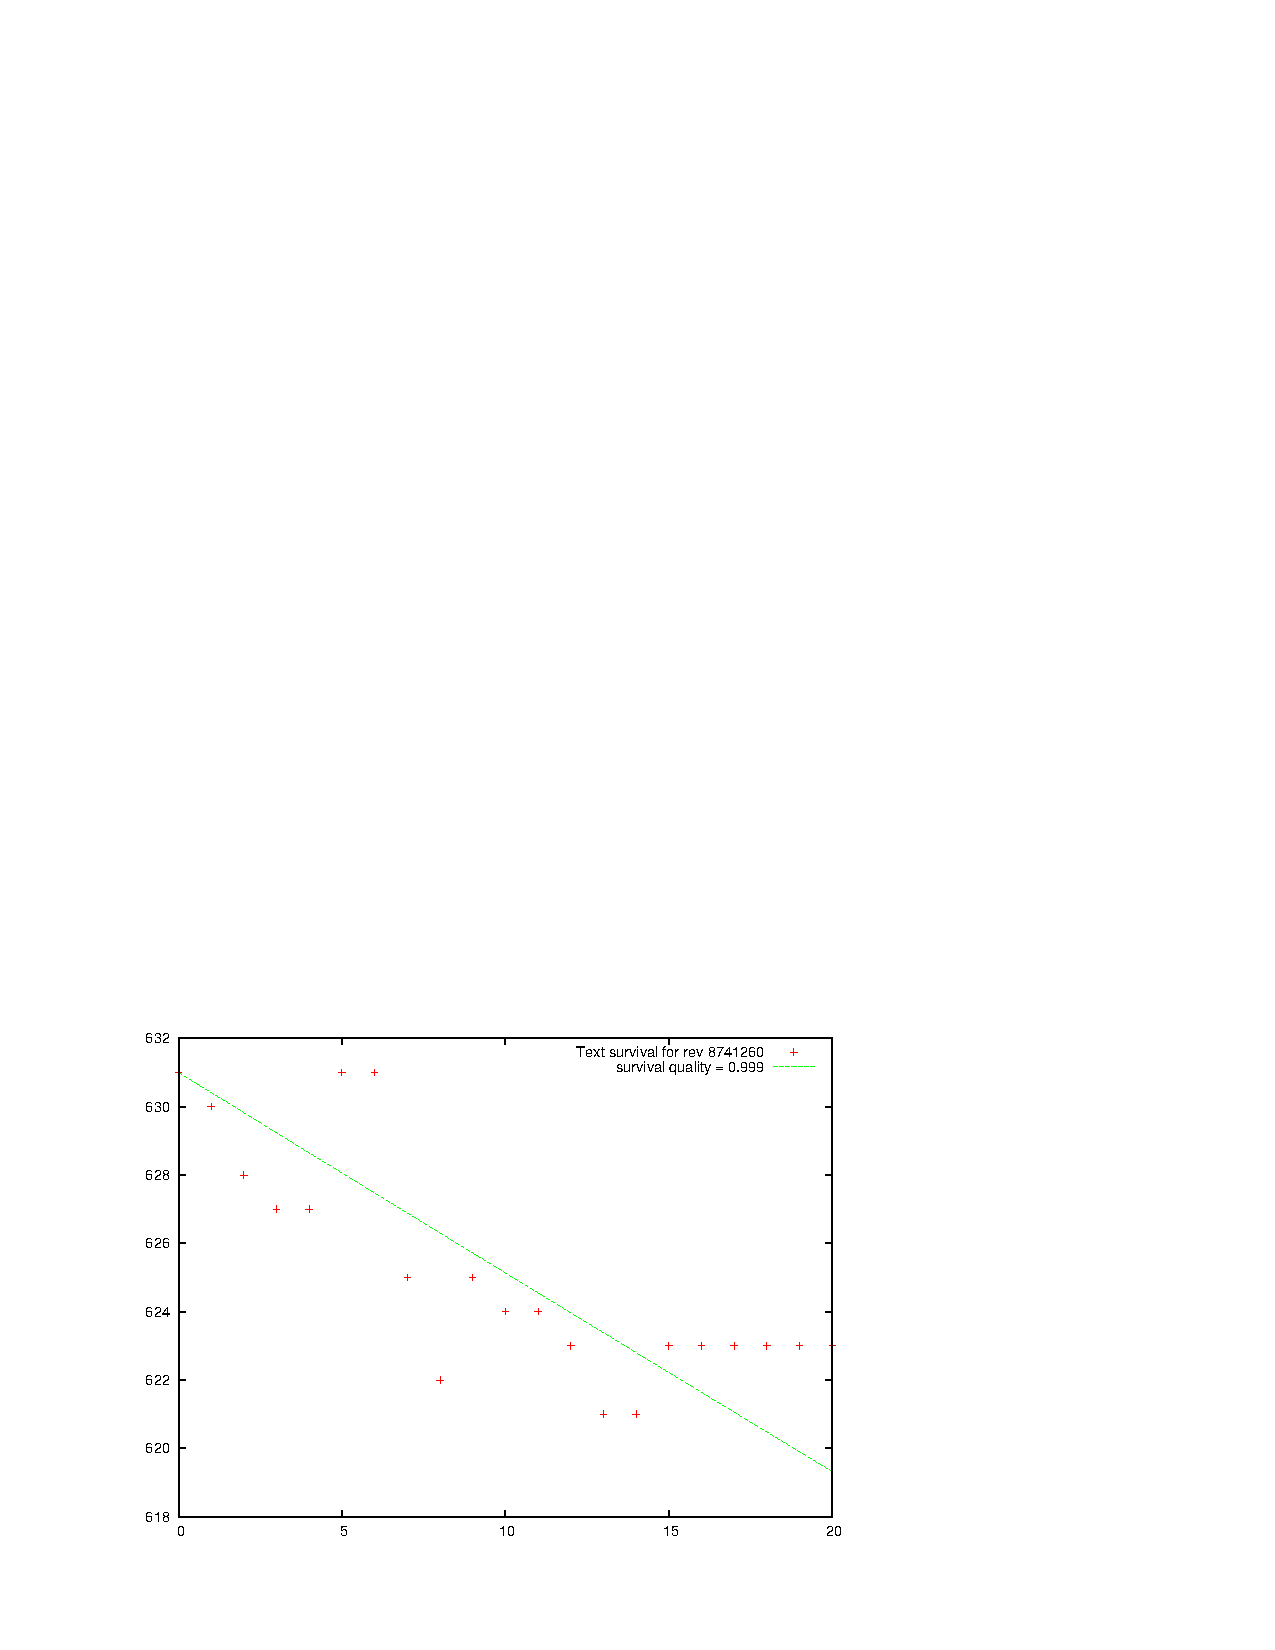
\includegraphics[width=0.8\textwidth]{part-F70-editquality/graph-TS-SantaCruzBeachBoardwalk}}
\caption{The text survival graph for the text initially contributed
	as part of the article \textit{Santa Cruz Beach Boardwalk}.
	The majority of the editing to the contributed text happens
	in the next few revisions, before the text stabilizes.
	The graph also shows the text survival quality
	computed based on 20~revisions.
	}
\label{fig:ts-SantaCruzBeachBoardwalk}
\end{figure}

The explanation for this discrepancy turns out to be a flaw in our
thinking about the original model.
While the text survival for contributions does seem to have an
exponential look to it, exponentials do not approach some fixed
non-zero value --- they approach zero.
In order to fit the curve we are describing, the last value
(in the case of the data shown in Figure~\ref{fig:ts-GeorgeWBush},
the amount of text that survives after the $20^{th}$ revision)
should be taken as the ``zero reference point'' which is subtracted
from all the values.
Applying our exponential curve fitting technique to these new values
will give a much better approximation to the data.
The problem with this better fit is that it changes the meaning of
a score of zero; instead of meaning that the text was immediately deleted,
a score of zero would mean that the text immediately reached its
final survival level.
In other words, we would be measuring how quickly the text stabilizes,
rather than how much agreement there was that the text belonged in
the article.

\subsection{The Triangle Inequality}

We previously noted that our formulation of edit longevity does
not precisely stay within the desired range of $[-1,+1]$,
because our use of a greedy differencing algorithm does not
guarantee the shortest edit script.
In order to quantify how often such an error might crop up,
we counted how many triangles were evaluated for our PAN-WVC-10
revisions, and how many of those fell outside of the range $[-1,+1]$.

\begin{table}[htbp]
\begin{center}
\begin{tabular}{|r|c|c|c|}
\hline
Diff & Edit Distance & Total Triangles & Bad Triangles \\
\hline
\hline
basic & initial distance & xx & xx \\
basic & updated distance & xx & xx \\
live & I+D+M & 850,060 & 46,740 \\
live & graph & 852,040 & 162,922 \\
\hline
\end{tabular}
\end{center}
\caption{Estimating how often the triangle inequality does
    not hold when evaluating edit longevity of the
    PAN-WVC-10 annotated revisions.
} 
\label{tbl:badtriangles}
\end{table}


